\documentclass[12pt]{article}
%%%%%%%%%%%%%%%%%%%%%%%%%%%%%%
%Force pdflatex processing even with "$ latex" (required by arXiv)
\pdfoutput=1
%%%%%%%%%%%%%%%%%%%%%%%%%%%%%
\usepackage[top=3cm, bottom=3cm, left=2cm, right=2cm]{geometry}
\usepackage[usenames,dvipsnames,svgnames]{xcolor}
\definecolor{darkblue}{rgb}{0.0,0.1,0.3} % dark blue
\definecolor{darkgreen}{rgb}{0,0.65,0}
\definecolor{dblue4}{rgb}{0.06,0.31,0.55} % DodgerBlue4
\definecolor{nicered}{rgb}{0.7,0.1,0.1}
\definecolor{nicegreen}{rgb}{0.1,0.5,0.1}

\usepackage[numbers,sort&compress]{natbib}
%\usepackage{cite}

\usepackage[utf8]{inputenc}
\usepackage{textcomp}
\usepackage{amsmath,amssymb,amsfonts,amsthm}
\usepackage{siunitx} 
\usepackage{tabularx}
\usepackage{multirow}
\usepackage{dsfont}
\newcolumntype{Y}{>{\centering\arraybackslash}X}

\usepackage{xcolor}
\usepackage[colorlinks=true,citecolor= nicegreen,linkcolor=nicered]{hyperref}

\usepackage{verbatim} 
\usepackage{graphicx}
\graphicspath{{figures/}}
\usepackage{cancel}

\usepackage[colorinlistoftodos]{todonotes}

\usepackage{comment}
\includecomment{details}
\specialcomment{details}
{\begingroup}{\endgroup}
\excludecomment{details}
%\PreviewEnvironment{details}
%%%%%%
%Custom definitions
\usepackage{tikz}
\newcommand{\ReportNumbers}[1]{%
\begin{tikzpicture}[overlay, remember picture]
\path (current page.north east) ++(-1,-1) node[below left] {#1};
\end{tikzpicture}
}
%%%%%%%%%%%%%%%TITLE PAGE

\title{Dirac neutrino mass generation from Majorana messenger}

\author{First Author\footnote{\href{mailto:first@author}{first@author}},
Second Author\footnote{\href{mailto:second@author}{second@author}}\\
\textit{\small  First Institute}\\
[4mm]
Third Author\footnote{\href{mailto:third@author }{third@author}}\\
\textit{\small Second Institute}
}
\date{\small Month NN, YYYY}
\begin{document}
\maketitle
\ReportNumbers{XXX-XXX}

\begin{abstract}    

We propose a two-Higgs-doublet model (THDM) for one-loop Dirac neutrino masses with Majorana mediators which can be dark matter candidates if they are the lightest states circulating the loop. This model is restricted by  neutrino physics,  lepton flavor violation and cosmological constrains, including  
the effective number light neutrinos $N_{\text{eff}}$ . Here we find that $M_{Z^{\prime}}/g^{\prime} \gtrsim 60\ \text{TeV}$ in order to satisfy the conditions of $N_{\text{eff}}$..
\end{abstract}

\section{Introduction}
\label{sec:intro}
%Dirac vs Majorana (From previous paper: must be rephrased
The interpretation of neutrino experimental data in terms of neutrino
oscillations is compatible with both Majorana or Dirac neutrino masses
\cite{Tanabashi:2018oca}. The former possibility has received the most
attention but, given the lack of signals in neutrinoless double beta
decay experiments
\cite{KamLAND-Zen:2016pfg,Agostini:2018tnm,Aalseth:2017btx,Alduino:2017ehq,Albert:2017owj,Arnold:2016bed},
the latter cannot be dismissed. If neutrinos are Dirac particles, the
Standard Model (SM) particle content must be extended with
right-handed neutrinos, which can increase the number the effective
number light neutrinos, $N_{\text{eff}}$, until 6. To give small
masses to at least two Majorana or Dirac neutrinos, as required to
explain the neutrino oscillation experiments~\cite{Ahmad:2002jz,
  Fukuda:1998mi}, the seesaw mechanism with heavy fermions is usually
invoked. For the tree-level type-I seesaw we can have either light Majorana neutrinos with heavy Majorana mediators~\cite{} or light Dirac neutrinos with heavy Dirac mediators~\cite{} (see provisional figure below). The radiative type-I seesaw includes these both possibilities:~\cite{} and \cite{}, but now it is possible also to have also Majorana fermions with Dirac mediators. In this
work we want to explore the possibility to build a simple model with
Dirac masses and Majorana mediators.

%TO BE DELETED
Preliminary discussion: At three level a Dirac seesaw with Majorana mediators automatically allows for Majorana masses, as illustrated in the provisional plot: neutrinos. See plot:

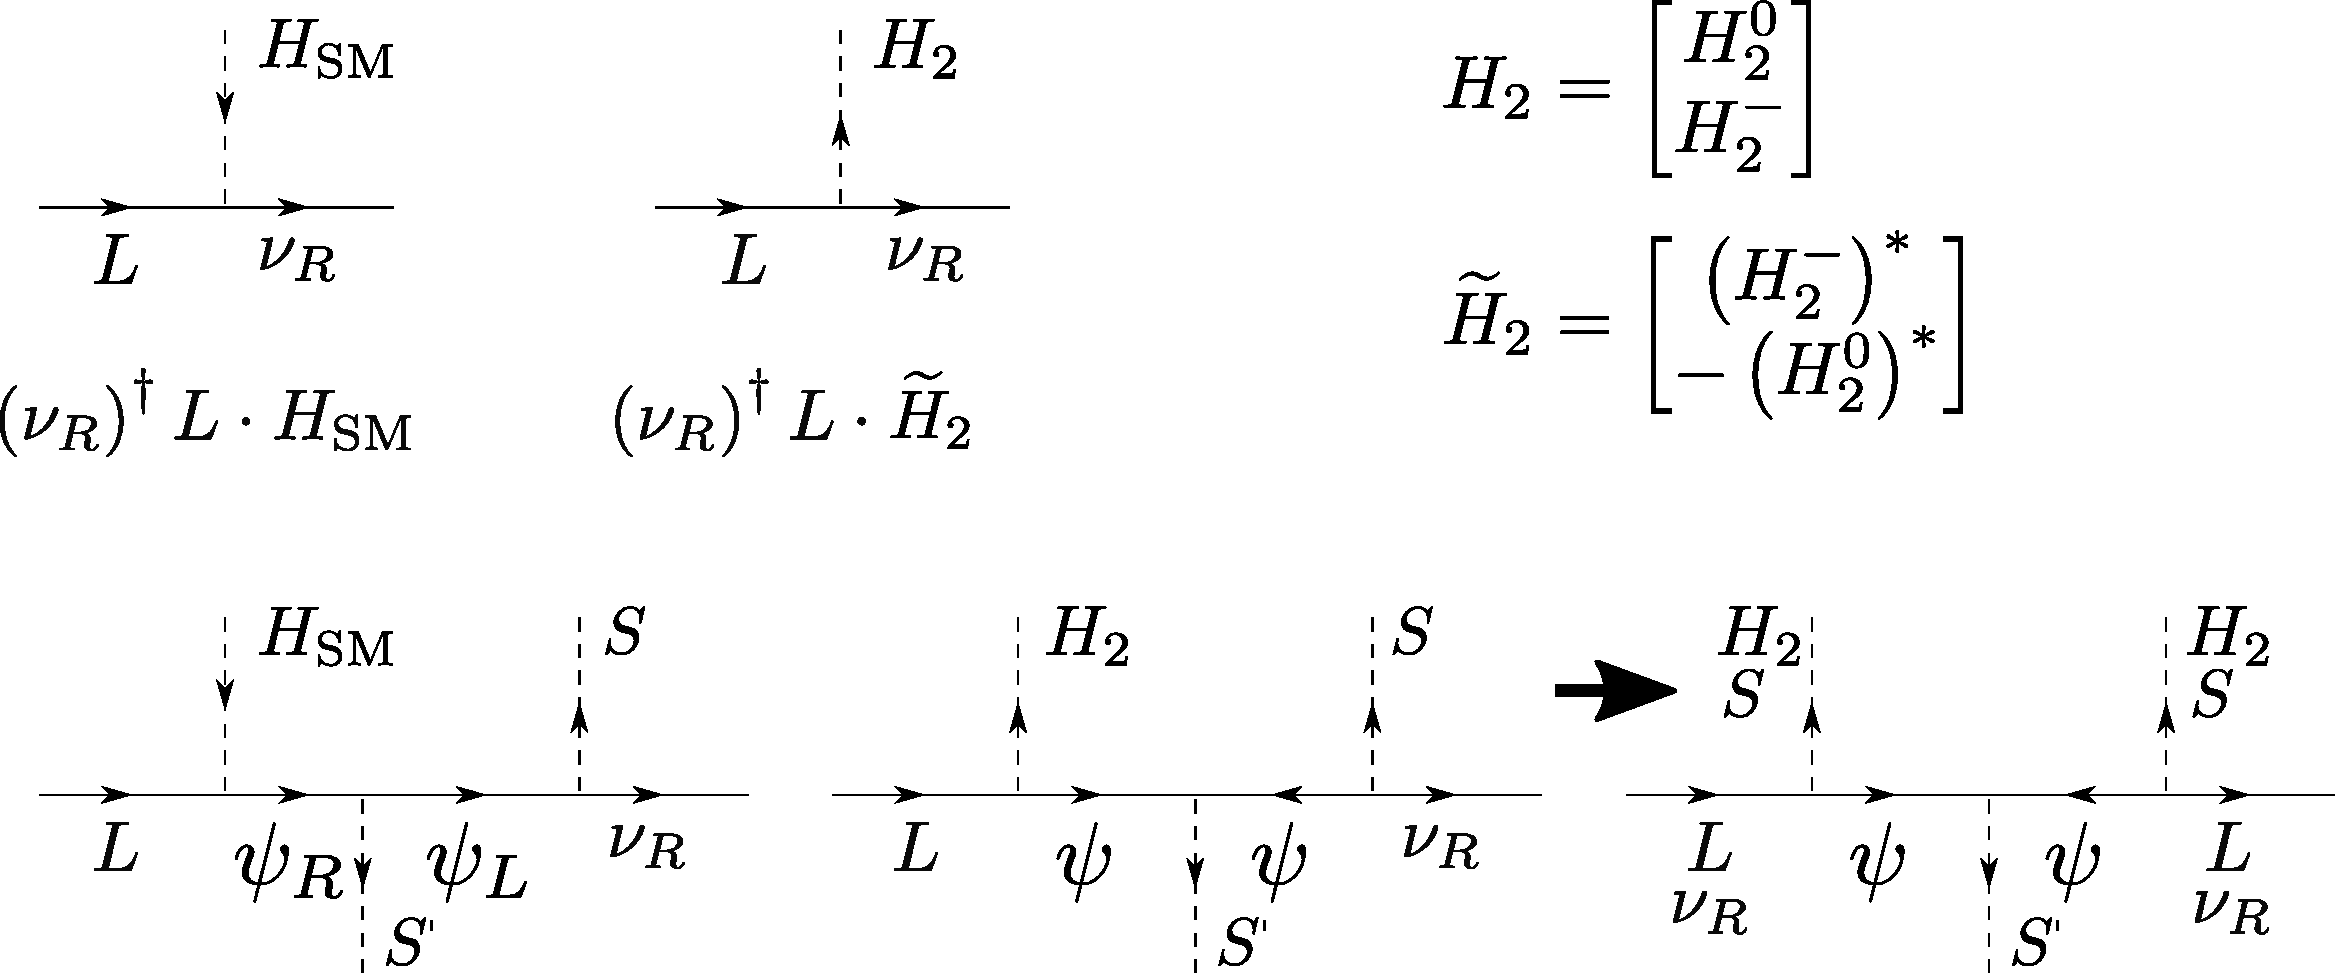
\includegraphics[scale=0.4]{tl}


% Tree-level see-saw with fermionic mediators: Dirac for Dirac, Majorana-Majorana
% One-loop level: Majorana-Majorana, Dirac-Dirac, Majorana-Dirac. Simplest model with Dirac-Majorana still missing
% At one-loop Dark Matter is predicted in model-dependent ways. In this case...



The standard model (SM) does not explain the neutrinos mass predicted by the neutrino oscillation experiments~\cite{Ahmad:2002jz, Fukuda:1998mi}. From neutrino oscillation experiments, we know that at least two neutrinos must be massive and their respective mixing angles~\cite{deSalas:2017kay}. The experiments still do not determine if the neutrinos are Dirac or Majorana particles, since the double beta decays are not yet conclusive~\cite{Arnold:2016bed, Albert:2017owj, Alduino:2017ehq, Aalseth:2017btx, Agostini:2018tnm, KamLAND-Zen:2016pfg}.

In the SM all fermions acquire masses through a Dirac term, it is natural to believe that neutrinos acquire masses in this way, so there are some studies that develop this hypothesis~\cite{Branco:1978bz}. If the neutrinos are  Dirac, this establishes a physics beyond SM (BSM), this predicts the existence of at least two right-handed neutrinos. If neutrino mass is generated at tree level, establishes that Yukawas must be very small ($\lesssim 10^{-10}$) to explain tiny neutrino masses~\cite{deSalas:2017kay}. So it is preferred to generate the masses through mechanisms that develop in a loop~\cite{Branco:1978bz, Zee:1980ai, Ma:2006km}.

In some models to forbidden terms of Dirac at tree level and Majorana terms, discrete ad hoc symmetries are added~\cite{Han:2018zcn, Wang:2017mcy}. In recent works, using symmetry ($B-L$) to forbid these terms without resorting to discrete symmetries~\cite{Calle:2018ovc, Bonilla:2018ynb, Saad:2019bqf}. In these cases, it is necessary to introduce new scalars and new dirac or vector-like fermions, that are used for to close the loop.

Another evidence that SM is not a complete theory is the missing mass in the universe, which is known as dark matter (DM). The main proposals that explain DM as a particle are given in Ref.~\cite{Bertone:2004pz}. We will make use of the scotogenic model~\cite{Ma:2006km}. In scotogenic model the neutrino masses and the DM have common explanation. The mass of the neutrinos is generated to one-loop, where the mediators in the loop are viable candidates for DM.

In this work we propose a model with Dirac neutrinos at one-loop, in which the mediators are Majorana fermion and one singlet scalar and one doublet scalar. This mediators can to be dark matter candidates. Additionally, for generated neutrino mass is necessary to add a second Higgs doublet. The rest of the paper is organized as follows. In the next section we present the model and the particle content. In the section~\ref{sec:ScaMassSpect} we study the scale mass spectrum after spontaneous symmetry breaking. In section~\ref{sec:Neutrinos} we present the mechanism that generates the neutrino masses. In section~\ref{sec:LFV} we show the experimental lepton flavor violation (LFV) constrains. Finally, in the section~\ref{sec:DM} we present the viable DM candidates.

\section{The model}
\label{sec:Model}
As a preliminary model, we propose a model that includes an additional Higgs doublet with $ Y = -1/2 $. The two doublets are coupling differently to the fermions, the first doublet is coupled to quarks up-type and the charged leptons, while the second doublet is coupled to down-type quarks. To forbid another terms, we used a $U(1)^{\prime}$ symmetry. This model is known as two Higgs doublets model type II (2HDM-II)~\cite{Davidson:2005cw}. Also, these symmetry allows us to forbid Dirac mass terms at tree level. Additionally, we add three right neutrinos, one scalar doublet, two scalar singlets and three Majorana fermion singlet under $SU(2)_L$. The $U(1)^{\prime}$ charge for the new particles will be defined by the anomaly cancellation equations and the Yukawa interactions. In this model the neutrinos are Dirac fermions. Particle content and their respective charges are show in Tab.~\ref{tab:partcont}. 

The most general Yukawa Lagrangian is:
%
\begin{align*}
\label{Eq:LagY}
    \mathcal{L} \subset& -[ 
    h^{a}_{i} \overline{L_{i}} \psi_{a} \widetilde{\eta}  +  y^{a}_{j} \overline{\nu_{R_{j}}} \sigma \psi_{a} + y_{\psi}^{a b} \overline{\psi^{c}_{a}} \psi_{b} S^{*} + h.c.] \\
    &- \mathcal{V}(H_{u}, H_{d}, S, \eta, \sigma)\,,
\end{align*}
%
where $L_{i}$ are the SM lepton doublets, $\eta = \left( \eta^{+} \ \eta^{0} \right)^{T}$, $\widetilde{\eta} = i \sigma_2 \eta^{*}$ and $\mathcal{V}(H_{u}, H_{d}, S, \eta, \sigma)$ is the scalar potential. $h^{a}_i$ and $y^{a}_{j}$ ($i,j,a=1,2,3$) are matrix in flavor space.
%
\begin{table}
  \centering
  \begin{tabular}{|l|l|l|}
    \hline  
    Particles     & $\left( SU(2)_L, U(1)_Y \right)$ & $U(1)^{\prime}$ \\ \hline
    $H_{d} $  & $(2,-1/2)$ &  2 \\
    $H_{u} $  & $(2, 1/2)$ &  0 \\
    $\eta$ & $(2,1/2)$ & $-1$ \\
    $S$ & $(1,0)$ & $-2$ \\
    $\sigma$ & $(1,0)$ & $-3$ \\
    \hline
    $Q_{L_{i}}$  & $(2,-1/6)$ & $0$ \\
    $\overline{u_{R_{i}}}$ & $(1,-2/3)$ & $0$ \\
    $\overline{d_{R_{i}}}$ & $(1,1/3)$ & $-2$ \\
    \hline
    $L_i$  & $(2,-1/2)$ & $0$ \\
    $\overline{e_{R_i}}$ & $(1,1)$ & $0$ \\
    $\overline{\nu_{R_{i,j}}}$ & $(1,0)$ & $4$\\
    $\overline{\nu_{R_k}}$ & $(1,0)$ & $-5$\\
    $\psi_{i}$  & $(1,0)$ & $-1$ \\\hline
  \end{tabular}
  \caption{Scalars and left-handed fermions with their respective charges.}
  \label{tab:partcont}
\end{table}
%

The most general gauge invariant scalar potential for this model is
%
\begin{align*}
    \mathcal{V}(H_{u}, H_{d}, S, \eta, \sigma) = & \mathcal{V}(H_{u}) + \mathcal{V}(H_{d}) + \mathcal{V}(S) + \mathcal{V}(\eta) + \mathcal{V}(\sigma) \\
    &+ \lambda_{1} (H^{\dagger}_{u} H_{u}) (H^{\dagger}_{d} H_{d}) + \lambda_{2} (H^{\dagger}_{u} H_{d}) (H^{\dagger}_{d} H_{u}) + \lambda_{3} (H_{u}^{\dagger} H_{u} ) (S^{*} S) + \lambda_{4} (H_{u}^{\dagger} H_{u} ) (\sigma^{*} \sigma ) \\
    &+ \lambda_{5} (H_{u}^{\dagger} H_{u} ) (\eta^{\dagger} \eta ) + \lambda_{6} (H_{d}^{\dagger} H_{d} ) (S^{*} S) + \lambda_{7} (H_{d}^{\dagger} H_{d} ) (\sigma^{*} \sigma ) + \lambda_{8} (H_{d}^{\dagger} H_{d} ) (\eta^{\dagger} \eta )  \\
    &+ \lambda_{9} (S^{*} S) (\sigma^{*} \sigma ) + \lambda_{10} (S^{*} S) (\eta^{\dagger} \eta ) + \lambda_{11} (\eta^{\dagger} \eta ) (\sigma^{*} \sigma ) + \lambda_{12} (\eta^{\dagger} H_{u} ) (H^{\dagger}_{u} \eta ) \\
    &+ \lambda_{13} (\eta^{\dagger} H_{d} ) (H^{\dagger}_{d} \eta ) + (\mu \epsilon_{a b} H_{d}^{a} \eta^{b} \sigma + \mu_{1} \widetilde{H^{\dagger}_{d}} H_{u} S + \text{h.c.})\,,
\end{align*}
%
where $\mathcal{V}(\omega) = \mu^{2}_{\omega} \omega^{\dagger} \omega + \lambda_{\omega} (\omega^{\dagger} \omega)^{2}/2$. We consider that the parameters are real, since we are not going to deal with the CP violation~\cite{Abe:2016sqa}.

\section{Scalar mass spectrum}
\label{sec:ScaMassSpect}

 After spontaneous symmetry breaking, both Higgs doublet and scalar $S$ can to acquire vev's
%
\begin{align*}
    H_{u} =& \begin{pmatrix}0 \\ \frac{1}{\sqrt{2}} (h+\upsilon_{1}) \end{pmatrix} \,,
    &H_{d} =& \begin{pmatrix}\frac{1}{\sqrt{2}} (H+\upsilon_{2}+iA_{0}) \\ h^{-} \end{pmatrix} \,, &S =& \frac{1}{\sqrt{2}} (\phi+\upsilon_{s})
    &\eta =& \begin{pmatrix}\eta^{+} \\ \eta^{0} \end{pmatrix} \,,
\end{align*}
%
with $\eta^{0} = (\eta_{1}^{0}+i \eta_{2}^{0})/\sqrt{2}$ and $\sigma = ({\sigma}_{1}+i {\sigma}_{2})/\sqrt{2}$ and $\langle  H_{i} \rangle = \upsilon_{i}$ with $\upsilon=\sqrt{\upsilon_{1}^2+\upsilon_{2}^2} \simeq 246$\,GeV. It's possible to parameterize the ratio of these vev's as $\tan \beta = \upsilon_{2}/\upsilon_{1}$.

With the minimum of the scalar potential it is possible to write $\mu_{H_{u}}^{2}$,$\mu_{H_{d}}^{2}$ and $\mu^{2}_{s}$ in terms of the other parameters the following way
%
\begin{align*}
    \mu^{2}_{H_{u}} =& -\frac{\upsilon^{2}}{2}\left[ 2 \lambda_{H_{u}} c^{2}_{\beta} - 2 t^{2}_{\beta} \left(\frac{\mu^{2}_{H_{d}}}{\upsilon^{2}}+\lambda_{H_{d}} s^{2}_{\beta} \right) + \left( \lambda_{3} - \lambda_{6} t^{2}_{\beta} \right) \frac{\upsilon^{2}_{s}}{\upsilon^{2}} \right]\,, \\
    \mu_{1} =& -\frac{\upsilon^{2}}{\sqrt{2}} \left[ \left( \frac{2\mu^{2}_{H_{d}}}{\upsilon_{s}} + \lambda_{6} \upsilon_{s} \right) \frac{s_{\beta}}{\upsilon_{1} \upsilon} + \left( (\lambda_{1}+\lambda_{2})c^{2}_{\beta} + 2 \lambda_{H_{d}} s^{2}_{\beta} \right) \frac{t_{\beta}}{\upsilon_{s}} \right]\,, \\
   \mu^{2}_{s} =& -\frac{\upsilon^{4}}{2 \upsilon^{2}_{s}} \left[ -2s^{2}_{\beta} \left( \lambda_{H_{d}} s^{2}_{\beta} + \frac{\mu^{2}_{H_{d}}}{\upsilon^{2}_{s}}\right) + \left( \frac{\lambda_{3}}{\upsilon^{2}} - (\lambda_{1}+\lambda_{2})s^{2}_{\beta} \right) c^{2}_{\beta} + 2 \lambda_{6} \frac{\upsilon^{4}_{s}}{\upsilon^{4}} \right]\,,
\end{align*}
%
where $t_{\beta} = \tan \beta$, $c_{\beta} = \cos \beta$ and $s_{\beta} = \sin \beta$. This allows to reduce the number of free parameters.

Of the original sixteen scalar degrees of freedom in the model, $W^{\pm}$, $Z^{0}$ and $Z^{\prime}$ absorbed four of these (Goldstone bosons $G^{\pm}$,$G^{0}$ and $G^{\prime}$). There are two physical neutral CP-even Higgs state ($H$ and $h$, where $m_{H} \geq m_{h}$), one scalar state ($\phi$), one physical CP-odd Higgs scalar ($A^{0}$), two CP-even scalar state ($\sigma_{1}$ and $\eta^{0}_{1}$), two CP-odd scalar state ($\sigma_{2}$ and $\eta^{0}_{2}$), one charged scalar pairs ($\eta^{\pm}$) and one charged Higgs pairs ($h^{\pm}$). The mass spectrum for the scalar sector is given by
\begin{align*}
    m_{h^{\pm}}^{2} &= \mu^{2}_{H_{d}} + \frac{1}{2}(\lambda_{1} \upsilon^{2}_{1} + 2\lambda_{H_{d}} \upsilon^{2}_{2} + \lambda_{6} \upsilon^{2}_{s})\,, \\
    m_{\eta^{\pm}}^{2} &= \mu_{\eta}^{2} + \frac{1}{2} (\lambda_{5} \upsilon^{2}_{1} + \lambda_{8} \upsilon^{2}_{2} + \lambda_{10} \upsilon^{2}_{s} )\,, \\
    m_{A^{0}}^{2} &= m_{h^{\pm}}^{2} + \frac{1}{2} \lambda_{2} \upsilon^{2}_{1} \,,
\end{align*}
%
note that the two charged scalars do not mix among themselves. The neutral mass eigenstate are defined as
%
\begin{align*}
    \begin{pmatrix}\chi_{(R,I)_{1}} \\ \chi_{(R,I)_{2}} \end{pmatrix} =& \begin{pmatrix} c_{\theta_{(R,I)}} & -s_{\theta_{(R,I)}} \\ s_{\theta_{(R,I)}} & c_{\theta_{(R,I)}} \end{pmatrix} \begin{pmatrix}\sigma_{(1,2)} \\ \eta_{(1,2)} \end{pmatrix} \,,
\end{align*}
%
where $\tan2\theta_{(R,I)} = \pm2c/(b-a)$ and we defined $a = \mu^{2}_{\sigma}+\frac{1}{2}(\lambda_{4} \upsilon^{2}_{1} + \lambda_{7} \upsilon^{2}_{2} + \lambda_{9} \upsilon^{2}_{s})$\,,
$b = \mu^{2}_{\eta^{\pm}} + \frac{1}{2}(\lambda_{12} \upsilon^{2}_{1} + \lambda_{13} \upsilon^{2}_{2})$ and $c = \mu \upsilon_{2}/\sqrt{2}$\,. The corresponding mass eigenvalues are
\begin{align*}
    m_{\chi_{R(1,2)}}^{2} &= \frac{1}{2} \left(a + b \mp \sqrt{(a-b)^{2} + 4c} \right)\,, \\
     m_{\chi_{I(1,2)}}^{2} &= \frac{1}{2} \left(a + b \mp \sqrt{(a-b)^{2} - 4c} \right)\,,
\end{align*}

\section{Neutrinos}
\label{sec:Neutrinos}
%
\begin{figure}
\centering
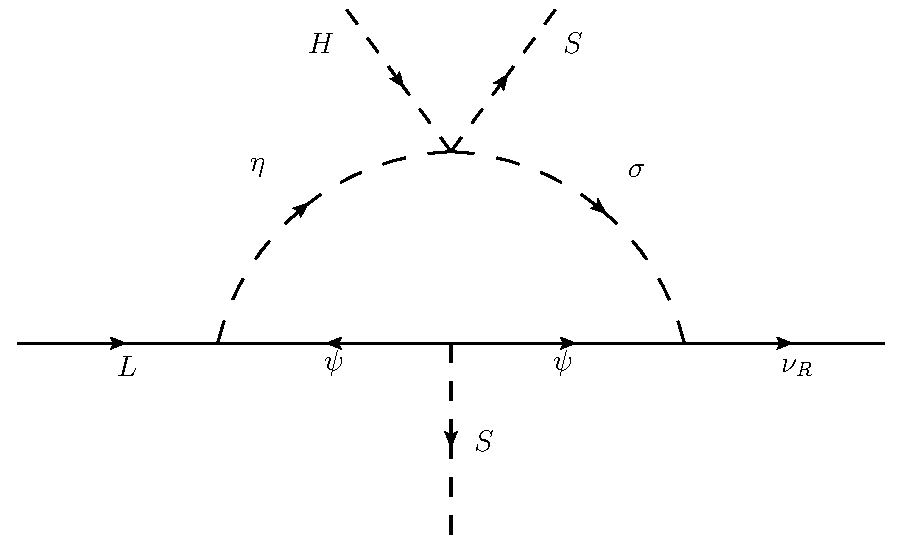
\includegraphics[scale=0.75]{Neutrino_Loop.pdf}
\caption{One-loop generation of Dirac neutrino mass}
\label{fig:zee}
\end{figure}
%
 The Dirac neutrino mass matrix in this model is generate to one loop level, which is shown in fig(\ref{fig:zee}). The expression for $\mathcal{M}_{\nu}$ is given by~\cite{Reig:2018mdk}
%
\begin{align}
(\mathcal{M}_{\nu})_{ij} = \frac{\sqrt{2}\mu \upsilon_{2}}{64 \pi^{2}} \sum_{a=1}^{3} \frac{h_{i}^{a} M_{\psi_{a}}y_{j}^{a}}{m_{\chi_{R2}}^{2}-m_{\chi_{R1}}^{2}} \left[ F\left( \frac{m_{\chi_{R2}}^{2}}{M_{\psi_{a}}} \right) - F\left( \frac{m_{\chi_{R1}}^{2}}{M_{\psi_{a}}} \right) \right] + (R \to I)\,,
\end{align}
%
where $F(m_{S_{\beta}}^{2}/M_{\psi}^{2}) = m_{S_{\beta}}^{2}\log(m_{S_{\beta}}^{2}/M_{\psi})/(m_{S_{\beta}}^{2}-M_{\psi})$ is loop function, $M_{\psi_{a}}$ is the fermión mass  and $\chi_{R_(1,2)}$ are the two CP-even mass eigenstate and $\chi_{I_{(1,2)}}$ are two CP-odd mass eigenstate.To obtain neutrino masses it is necessary that $\mu \neq 0$. In addition, To explain the suppression of the mass matrix, it is usually assumed that the mass of the mediator fermions is very large. Another possibility is small values of $\mu$, this suppress the value of the neutrino masses. The structure of the effective neutrino mass matrix is given by the product $(M_{\nu})_{ij} \propto h^{a}_{i} y^{b}_{j}$, which is similar to the structure of the neutrino mass matrix for the tree-level seesaw mechanism for Dirac neutrinos~\cite{Chulia:2016ngi}. If only one fermion $\psi$ is added, we will have two massless neutrinos, which does not agree with the current data obtained from the neutrino experiments~\cite{deSalas:2017kay}. In our case, we will assume the existence of three fermions, generating Dirac scotogenic masses for the two neutrinos ($\nu_{k}$ is massless due to the assignment of charges).

For the Dirac neutrinos the mass matrices are diagonalized by
\begin{align}
(U^{(\nu)}_R)^{\dagger} M_{\nu_{D}} U^{(\nu)}_L = M_{\nu_{D}}^{\text{diag}} = \text{diag}(m1, m2, m3)\,,
\end{align}
where $U^{(\nu)}_R$ and $U^{(\nu)}_L$  are unitary $3 \times 3$ matrices. In the most general Dirac neutrino mass matrices, lepton mixing matrix is
\begin{align}
U_{\text{PMNS}} = (U^{(\ell)}_L)^{\dagger} U^{(\nu)}_L\,.
\end{align}
If we work in the basis where $\ell$ and $\nu_{R}$ are mass eigenstate, the matrices $U_{L}^{(\ell)} = U_{R}^{\nu} = \mathds{1}$. Therefore, we can to express the Dirac neutrino mass matrix following way
\begin{align}
(M_{\nu_{D}})_{ij} = (U_{\text{PMNS}})_{ij} (M_{\nu_{D}}^{\text{diag}})_{jj}\,,
\end{align}
where the matrix $U_{\text{PMNS}}$ is expressed in the standard parameterization as
\begin{align}
U_{\text{PMNS}} = \begin{pmatrix}
    1 & 0		& 0 \\
    0 & c_{23}  & s_{23} \\
    0 & -s_{23} & c_{23}
\end{pmatrix}
\begin{pmatrix}
    c_{13}  &  0 & s_{13}e^{-i\delta} \\
    0 		&  1 & 0 \\
    -s_{13}e^{i\delta} &  0 & c_{13}
\end{pmatrix}
\begin{pmatrix}
    c_{12}  & s_{12} & 0 \\
    -s_{12} & c_{12} & 0 \\
    0		& 0		 & 1
\end{pmatrix}\,,
\end{align}
where $s_{ij} = \sin \theta_{ij}$ and $c_{ij} = \cos \theta_{ij}$ and $\theta_{ij}$ are neutrino mixing angles.

\section{Lepton flavor violation}
\label{sec:LFV}
%
\begin{figure}
\centering
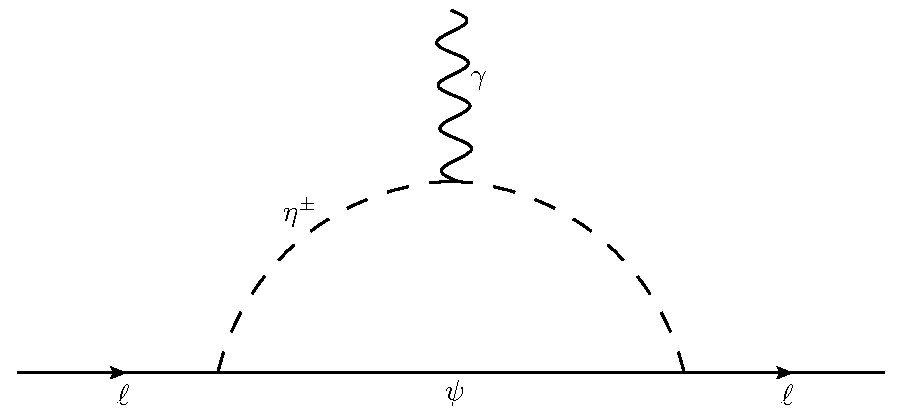
\includegraphics[scale=0.6]{LFV.pdf}
\caption{Feynman diagram for process $l^{-}_{i} \to l^{-}_{j} \gamma$}
\label{fig:LFV}
\end{figure}
%
The new Yukawa interactions in Eq~\eqref{Eq:LagY} in our model introduce processes that violate the leptonic flavor in the charged sector (CLFV). These CLFV processes are induced at one loop level, as shown in the figure~\ref{fig:LFV}. In this case, the $\psi_{a} \widetilde{\eta}^{\dagger} L_{i}$ interaction allows the part of the double scalar $\eta$ ($\eta^{\pm}$) to mediate in the loop.

The most common search for CLFV focuses on the $l^{-}_{i} \to l^{-}_{j} \gamma$ process. This process is described by the effective Lagrangian
%
\begin{align}
    \mathcal{L} = \frac{\mu_{m}^{\alpha \beta}}{2} l^{-}_{\beta} \sigma^{\mu \nu} l^{-}_{\alpha} F_{\mu \nu}
\end{align}
%
where $\mu_{m}^{\alpha \beta}$ is a transition magnetic moment~\cite{Toma:2013zsa}.
The decay rate is given by~\cite{Lavoura:2003xp}
%
\begin{align}
 \Gamma(l^{-}_{i} \to l^{-}_{j} \gamma) = \frac{m^{3}_{i}}{16 \pi} \left| \sum_{\alpha} h^{\alpha}_{i} m_{i} h^{\alpha}_{j} \frac{i e}{16 \pi M^{2}_{\eta^{-}}} K(t_{k}) \right|^{2}\,, 
\end{align}
%
where $t_{\alpha} = M^{2}_{\psi_{\alpha}}/M^{2}_{\eta^{-}}$ and
%
\begin{align}
    K(t_{\alpha}) = \frac{2t_{\alpha}^{2}+5t_{\alpha}-1}{12(t_{\alpha}-1)^{3}} - \frac{t_{\alpha}^{2}\log t_{\alpha}}{2(t_{\alpha}-1)^{4}}\,.
\end{align}
%
If we assume that $t_{\alpha} \to 0$, $t_{\alpha} \to 1$ and $t_{\alpha} \to \infty$, we have that $K(t_{\alpha}) = 1/12$, $K(t_{\alpha}) = 1/24$ and $K(t_{\alpha}) = 1/(6t)$, respectively.

For $i \neq j$ we have CLFV processes. These processes are severely restricted by the current bounds , which set limits to the Yukawas. The most restrictive experimental bounds is decay $\mu \to e \gamma$, which is several orders of magnitude greater than radiative decays $\tau \to~l\gamma$, with $l = e, \mu$. These restrictions are given by Br$(\mu \to e\gamma)$ \textless $5.3 \times 10^{-13} $~\cite{Adam:2013mnn}, Br$(\tau \to e\gamma) $\textless$ 3.3 \times 10^{-8}$ and Br$(\tau \to~\mu\gamma) $\textless$ 4.4 \times 10^{-8}$~\cite{Aubert:2009ag, Bona:2007qt, Miyazaki:2012mx}. 

For $i = j$ we have processes that contribute to the leptonic magnetic dipole moment. In the case of the anomalous muon magnetic dipole moment, the experimental measurements do not agree with the values predicted by the SM~\cite{Lindner:2016bgg}. This can be a proof of the veracity of the model, in addition to giving restrictions on the Yukawas.

\section{Dark matter}
\label{sec:DM}
Depending on the the new particles mass hierarchy (scalars and fermions charged odd under $U(1)^{\prime}$), it is possible to have two candidates for DM. The first DM candidate is the lightest majorana fermion (assuming that $\psi_{1} < \psi_{2} < \psi_{3}$). The second candidate is scalar DM. The scalar that assumes the role of DM depends on which is the lightest scalar particle charged odd under $U(1)^{\prime}$. In this model the scalar DM can be the neutral component of the scalar doublet $\eta^{0}$ or the scalar singlet $\sigma$.

\subsection{Fermionic dark matter}
In the case that the mass of the lightest fermion $\psi$ is smaller than the mass of the scalars, the DM will be fermionic. For this DM it is possible to have the following observable decay of the scalar $\eta^{\pm} \to l^{\pm} \psi_{1}$, therefore, the other fermions decay as $ \psi \to l^{\pm} l^{\mp} \psi_{1}$ and $\psi \to l^{\pm} l^{\mp} \psi_{1,2} $, through $\eta^{\pm}$. The relic density of DM can be controlled by annihilation $\psi_{1} \psi_{1} \to l _{\alpha} \overline{l}_{\beta} $, via Yukawa coupling $h^{a}_{i}$. These Yukawa couplings are restricted under LFV and neutrino masses. But, Yukawa couplings $y^{a}_{j}$ is free.

Because the particle $\psi_{1}$ only interacts with the leptons via the Yukawa links and this particle does not interact with gluons and quarks, this model has no direct detection restrictions for DM. In the case where the mass of the other fermions and scalars is nearly degenerated to $\psi_{1} $, the processes of coaniquilación are relevant in relic density~\cite{Klasen:2013jpa}.

\subsection{Scalar dark matter}
For scalar DM we have that the lightest scalar charged odd under $U(1)^{\prime}$ must have a mass smaller than the lightest $\psi$ fermion. Contrary to fermionic DM, scalar DM has additional interactions to Yukawa couplings (scalar and gauge interactions), which can be used to control relic density.

If the lightest scale is the neutral part of the scalar doublet, we will have that the DM will be similar to the model of the inert doublet~\cite{Honorez:2010re}. For the inert doublet model there are two mass regions for DM which can to reproduce adequately the relic density ($50$GeV \textless $m_{DM}$ \textless $70$GeV and $535$GeV \textless $m_{DM}$ \textless $20$TeV)~\cite{Garcia-Cely:2015khw}. In recent studies, these two regions are connected through use of a second doublet~\cite{Borah:2019aeq}. How we have in the model the Yukawa coupling, the decay $\psi_{i} \to l^{\pm} \eta^{\mp}$ is possible. In addition, decay is given via scalar interactions $\eta^{\pm} \to \eta^{0} + {W^{\pm}}$, where $W^{\pm}$ can be real or virtual and decay to leptons or quarks.

Now, if the lightest scale is the scalar singlet, the DM will be similar to the model in Ref.~\cite{Athron:2017kgt}. The mass range for the scalar singlet that produces the adequate relic density is between approximately the Higgs mass and about $300$GeV and masses above $1$TeV. For this model, the term in the Lagrangian $\sigma^{2} H^{2}_{i}$ is known as the \textquotedblleft Higgs portal\textquotedblright. This term generates interesting phenomenological consequences. Such as, thermal production of DM in the early universe~\cite{Yaguna:2008hd}, direct detection and $h \to \sigma \sigma$~\cite{Mambrini:2011ik}. In addition, this model has important contributions to cosmology, in phenomena such as inflation~\cite{Lerner:2009xg} and baryogenesis~\cite{Cline:2012hg}.

\section{Cosmological constrain}
\begin{comment}
%
\begin{figure}
\centering
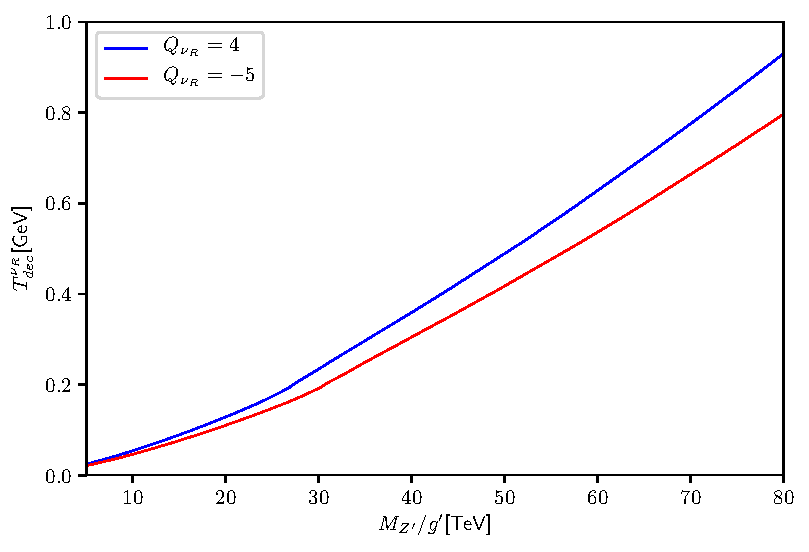
\includegraphics[scale=0.6]{Tdec.pdf}
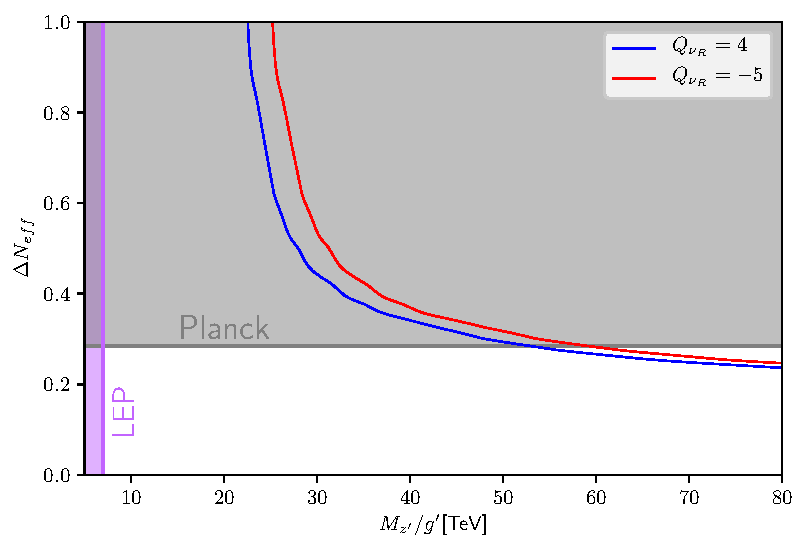
\includegraphics[scale=0.6]{Delta_Neff1.pdf}
\caption{One-loop generation of Dirac neutrino mass}
\label{fig:Neff}
\end{figure}
%
\end{comment}

The existence of three new right neutrinos in nature contribute to the total energy density of the universe. These new contributions can modify the cosmological observables in the CMB (cosmic microwave background). These new neutrinos contribute to the existence of dark radiation, which affects the expansion processes of the universe, which affects the number of relativistic degrees of freedom for neutrinos.

In the case of our models, this new gauge symmetry introduces a new gauge boson that mediates the interaction of the right neutrinos and the SM. This allows the right neutrinos to thermally modify the relativistic degrees of freedom, this contributions are given by~\cite{Anchordoqui:2012qu, Anchordoqui:2011nh}
%
\begin{align*}
    \Delta N_{eff} = N_{eff} - N^{SM}_{eff} = N_{\nu_R} \left( \frac{T_{\nu_{R}}}{T_{\nu_{L}}} \right)^{4} = N_{\nu_R} \left( \frac{g(T^{\nu_{L}}_{dec})}{g(T^{\nu_{R}}_{dec})} \right)^{4}
\end{align*}
%
where $ g(T) $ is the number of relativistic degrees of freedom at a temperature $T$ in the SM~\cite{Aghanim:2018eyx}. The decoupling temperature of the left neutrinos $\nu_L$ is $ T^{\nu_{L}}_{dec} \approx 2.3 $ MeV~\cite{Enqvist:1991gx}, when $g(T^{\nu_{L}}_{ dec}) = 43/4 $ corresponding to the three $\nu_{L}$, $e^{\pm} $ and the photon~\cite{Kolb:1990vq}. The rate of interaction of the right neutrinos with the SM is mediated by the gauge boson $Z^{\prime} $ and is given by~\cite{SolagurenBeascoa:2012cz}
%
\begin{align*}
    \Gamma_{\nu_R} (T) &= n_{\nu_R}(T) \langle \sigma(\overline{\nu_{R}} \nu_{R} \to \overline{f} f) \upsilon \rangle \,, \\
    &= \frac{g^{2}_{\nu_R}}{n_{\nu_R}(T)} \int \frac{d^{3} p}{(2 \pi)^{3}} f_{\nu_R}(p) \int \frac{d^{3} k}{(2 \pi)^{3}} f_{\nu_R}(k) \sigma_{f}(s) \upsilon\,,
\end{align*}
%
where $f_{\nu_R}(k)=1/(e^{k/T}+1)$ is the Fermi-Dirac distributión, $g_{\nu_R} = 2$ is spin number, $\upsilon = 1-\cos{\theta}$ is the Moller velocity, $s = 2 p k (1-\cos{\theta})$, where $p$ and $k$ are the momenta of the particle and $\theta$, the angle between them and the number density of right-handed neutrinos is given by
\begin{align*}
n_{\nu_R}(T) = g_{\nu_R} \int \frac{d^{3} k}{(2 \pi)^{3}} f_{\nu_R}(k)\,.
\end{align*}

The cross section is given in~\cite{Barger:2003zh}, in the case with heavy mediator $T^{\nu_R}_{dec} \ll M_{Z^{\prime}}$, we can to take the limit when $s \ll M_{Z^{\prime}}$ and neglecting the fermion masse, we have that the cross section is
%
\begin{align*}
    \sigma_{f}(s) \approx N^{C}_{f} \frac{s}{12 \pi} \left( \frac{g^{\prime}}{M_{Z^{\prime}}} \right)^{4} Q^{2}_{\nu_R} (Q^{2}_{f_L} + Q^{2}_{f_R})\,,
\end{align*}
%
where $N^{C}_{f}$ is the color multiplicity of the fermion, i.e. $N^{C}_{q(\ell)} = 3(1)$, $Q_{f}$ is the charge of the fermion under the new simmetry, $g^{\prime}$ and $M_{Z^{\prime}}$ are the gauge coupling and mass for the new gauge boson. Solving the integrals with this last cross section we obtain that the interaction rate is given by
%
\begin{align*}
    \Gamma_{\nu_{R}}(T) = \frac{49 \pi^{5} T^{5}}{97200 \zeta(3)} \left( \frac{g^{\prime}}{M_{Z^{\prime}}} \right)^{4} \sum_{f} N^{C}_{f} Q^{2}_{f}\,,
\end{align*}
%
%
\begin{figure}
\centering
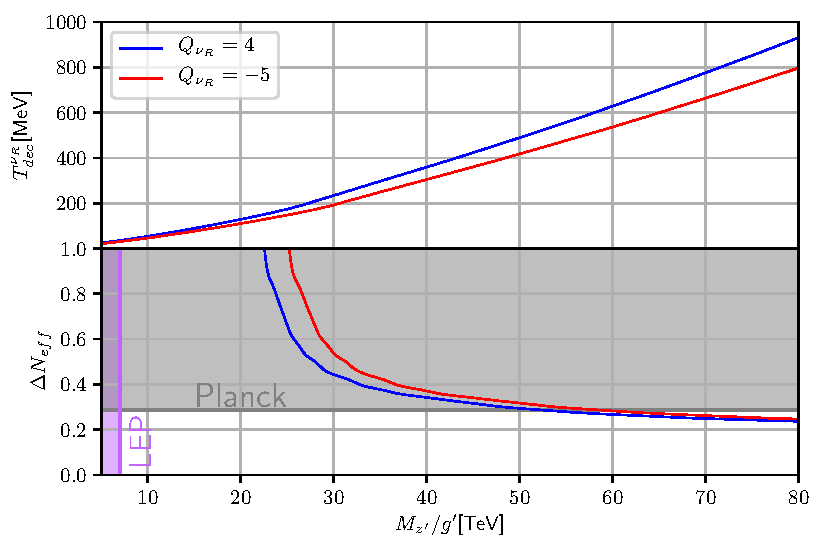
\includegraphics[scale=0.8]{DeltaNeff.pdf}
\caption{In the upper panel is the decoupling temperature of the right neutrino $\nu_{R}$ in function of $M_{z^{\prime}}/g^{\prime}$. In the lower panel is the additional contribution to the number of relativistic degrees of freedom ($\Delta N_{eff}$) in function of $M_{z^{\prime}}/g^{\prime}$. The gray shaded region is excluded by the measurements in the Planck CMB~\cite{Aghanim:2018eyx}. The region shaded in violet shows the bound from LEP  LEP~\cite{Alioli:2017nzr}.}
\label{fig:Neff}
\end{figure}
%
where the sum is performed over all SM fermion that are in thermal equilibrium with the plasma at temperature T. To estimate the contribution to relativistic degrees of freedom for neutrinos, it is necessary to calculate the decoupling temperature of the right neutrinos ($T^{\nu_R}_{dec}$). The latter occurs when the interaction rate of neutrinos with the SM drop below the rate of expansion of the universe, i.e.
%
\begin{align*}
\Gamma(T^{\nu_R}_{dec}) = H(T^{\nu_R}_{dec})\,, 
\end{align*}
%
where the Hubble expansion parameter is
%
\begin{align*}
    H(T) = \sqrt{\frac{8 \pi G_{N} \rho(T)}{3}} = \sqrt{\frac{4 \pi^{3} G_{N}}{45} \left( g(T) + \frac{21}{4} \right)} T^{2}\,,
\end{align*}
%
where $21/4$ correspond to the contribution of the right neutrinos to relativistic degrees of freedom. By finding the decoupling temperature of the right neutrinos $T^{\nu_R}_{dec} $ by a root finding method, it is possible to calculate $\Delta N_{eff}$.

The results of $T^{\nu_R}_{dec}$ and $\Delta N_{eff}$ as a function of $M_{Z^{\prime}}/g^{\prime}$ are exhibited in Fig~\ref{fig:Neff}. We can see that for small decoupling temperatures, the variation in the number of relativistic degrees of freedom of the new species is large and vice versa. The bound that come from Planck~\cite{ghanim:2018eyx}

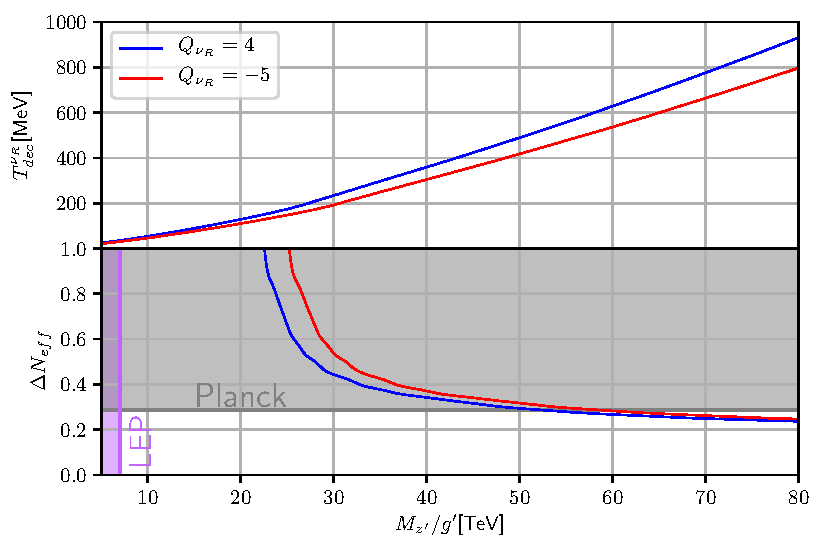
\includegraphics[scale=0.9]{DeltaNeff.pdf}

is stronger than the bound of LEP~\cite{Alioli:2017nzr}. For our model we find that $M_{Z^{\prime}}/g^{\prime} \gtrsim 60$TeV in order to satisfy the conditions of $N_{eff}$.

\appendix

%\bibliographystyle{h-physrev4}
%\bibliographystyle{JHEP-2}
%\bibliographystyle{JHEP}
\bibliographystyle{apsrev4-1long}
%\bibliographystyle{apsrev4-1longdoi}
\bibliography{susy}



\end{document}

%%% Local Variables: 
%%% mode: latex
%%% TeX-master: "draft"
%%% ispell-local-dictionary: "american"
%%% End: 
The cross section is given in [], in the case with heavy mediator $T^{\nu_R}_{dec} \ll M_{Z^{\prime}}$, we can to take the limit when $s \ll M_{Z^{\prime}}$ and neglecting the fermion masse, we have that the cross section is

